\documentclass{beamer}


\mode<presentation>
{
  \usetheme{CambridgeUS}
	\usecolortheme{beaver}
  % or ...

  \setbeamercovered{transparent}
  % or whatever (possibly just delete it)
}


\usepackage{xeCJK}
\usepackage{ulem}
\usepackage[english]{babel}
\usepackage[utf8]{inputenc}
\usepackage{times}
\usepackage[T1]{fontenc}
\usepackage{hyperref}
\usepackage{pifont}
\usepackage{biblatex}
\usepackage{bibentry}
\usepackage{verbatim}
\bibliography{cite}
\newcommand{\cmark}{\ding{51}}%
\newcommand{\xmark}{\ding{55}}%
\setCJKmainfont{WenQuanYi Micro Hei}
\renewcommand{\raggedright}{\leftskip=0pt \rightskip=0pt plus 0cm}
\raggedright

\let\oldfootnotesize\footnotesize
\renewcommand*{\footnotesize}{\oldfootnotesize\tiny}

\title[Intelligent Software Engineering] 
{Intelligent Software Engineering}
\subtitle{Requirements Engineering}

\author[Zhilei Ren] 
{Zhilei Ren}

\institute[Dalian University of Technology] % (optional, but mostly needed)
{
\\
\includegraphics[width=0.1\textwidth]{../utils/logo.png}\\
Dalian University of Technology
}


\subject{Software Engineering}



\pgfdeclareimage[width=0.08\textwidth]{university-logo}{../utils/logo.png}
\logo{\pgfuseimage{university-logo}}



% Delete this, if you do not want the table of contents to pop up at
% the beginning of each subsection:
\AtBeginSubsection[]
{
  \begin{frame}<beamer>{Outline}
    \tableofcontents[currentsection,currentsubsection]
  \end{frame}
}


% If you wish to uncover everything in a step-wise fashion, uncomment
% the following command: 

%\beamerdefaultoverlayspecification{<+->}

\setbeamertemplate{section in toc}[circle]
\setbeamertemplate{items}[circle]
\setbeamertemplate{caption}[numbered]
\setbeamertemplate{bibliography item}{\insertbiblabel}
\setbeamertemplate{bibliography entry title}{}
\setbeamertemplate{bibliography entry journal}{}

\begin{document}

\begin{frame}
  \titlepage
\end{frame}

%\begin{frame}{Outline}
%  \tableofcontents[currentsection,currentsubsection, 
%    hideothersubsections, 
%    sectionstyle=show,
%]
%\end{frame}

\AtBeginSection[]
{
 \begin{frame}<beamer>
 \frametitle{Outline}
 \tableofcontents[currentsection]
 \end{frame}
}
\begin{frame}[t]{Definition of Requirements Engineering}
    Requirements engineering is an interdisciplinary function that mediates between the domains of the acquirer and supplier or developer to establish and maintain the requirements to be met by the system, software or service of interest. Requirements engineering is concerned with discovering, eliciting, developing, analyzing, verifying (including verification methods and strategy), validating, communicating, documenting and managing requirements\footnote{ISO/IEC/IEEE 29148 Systems and software engineering — Life cycle processes -- Requirements engineering}.
\end{frame}

\begin{frame}[t]{As Proposed by the Project Sponsor}
    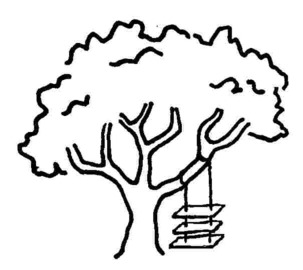
\includegraphics[width=.4\textwidth]{treemark.jpg} 
\end{frame}

\begin{frame}[t]{As Specified in the Project Request}
    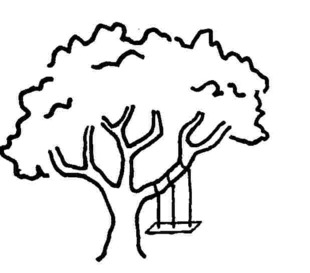
\includegraphics[width=.4\textwidth]{treemana.jpg} 
\end{frame}
\begin{frame}[t]{As Designed by the Senior Systems Analyst}
    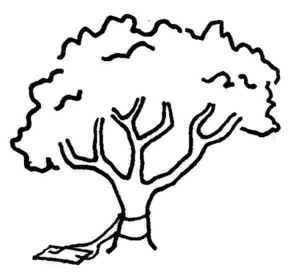
\includegraphics[width=.4\textwidth]{treeeng.jpg} 
\end{frame}
\begin{frame}[t]{As Produced by the Programmers}
    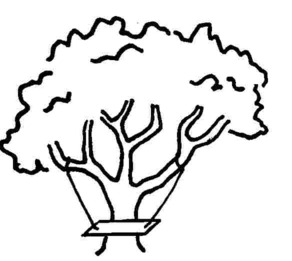
\includegraphics[width=.4\textwidth]{treemanu.jpg} 
\end{frame}
\begin{frame}[t]{As Installed at the User's Site}
    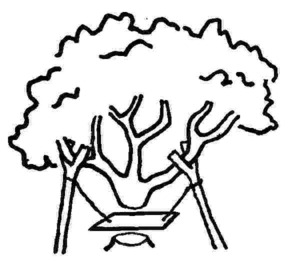
\includegraphics[width=.4\textwidth]{treemain.jpg} 
\end{frame}
\begin{frame}[t]{What The User Wanted}
    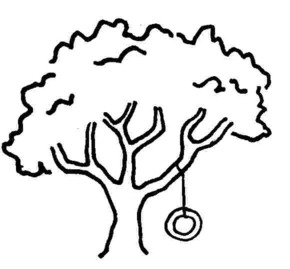
\includegraphics[width=.4\textwidth]{treecust.jpg}
\end{frame}

\begin{frame}[t]{Guide to Good Programming Practice, 1979}
    
\includegraphics[width=.4\textwidth]{treeswing_computer_book_cover.jpg}
\end{frame}

\begin{frame}[t]{Research Topics in Requirements Engineering}
    \begin{enumerate}
        \item Requirements Classification
        \item Requirements Prioritization
        \item Feature Model Optimization
        \item Prototype Generation
    \end{enumerate}
\end{frame}

\begin{frame}[t]{Techniques for Requirements Engineering Research}
\end{frame}

\begin{frame}[t]{Next Release Problem}
    % https://mde-optimiser.github.io/case-studies/nrp/
    % https://www.sciencedirect.com/science/article/pii/S095058490100194X
    % feature model
    Given:
    \begin{itemize}
      \item A set of software requirements \( R = \{r_1, r_2, \dots, r_n\} \),
      \item A set of customers \( C = \{c_1, c_2, \dots, c_m\} \),
      \item Each customer \( c_j \in C \) requests a subset of requirements \( R_j \subseteq R \) and provides a profit  \( p_j > 0 \) if all requirements in \( R_j \) are satisfied,
      \item Each requirement \( r_i \in R \) has an associated cost \( \text{cost}(r_i) > 0 \),
      \item A total available budget \( B > 0 \).
    \end{itemize}

    The goal is to select a subset of requirements \( R' \subseteq R \) such that:
    \begin{enumerate}
      \item The total cost does not exceed the budget: $\sum_{r_i \in R'} \text{cost}(r_i) \leq B$, 
      \item The total profit is maximized:
      \[
      \max_{R' \subseteq R} \sum_{\substack{c_j \in C \\ R_j \subseteq R'}} p_j.
      \]
    \end{enumerate}

    This is known as the \textbf{Next Release Problem (NRP)} and is a well-known NP-hard problem in requirements engineering and software release planning.
\end{frame}

\begin{frame}[t]{bug or feature?}
    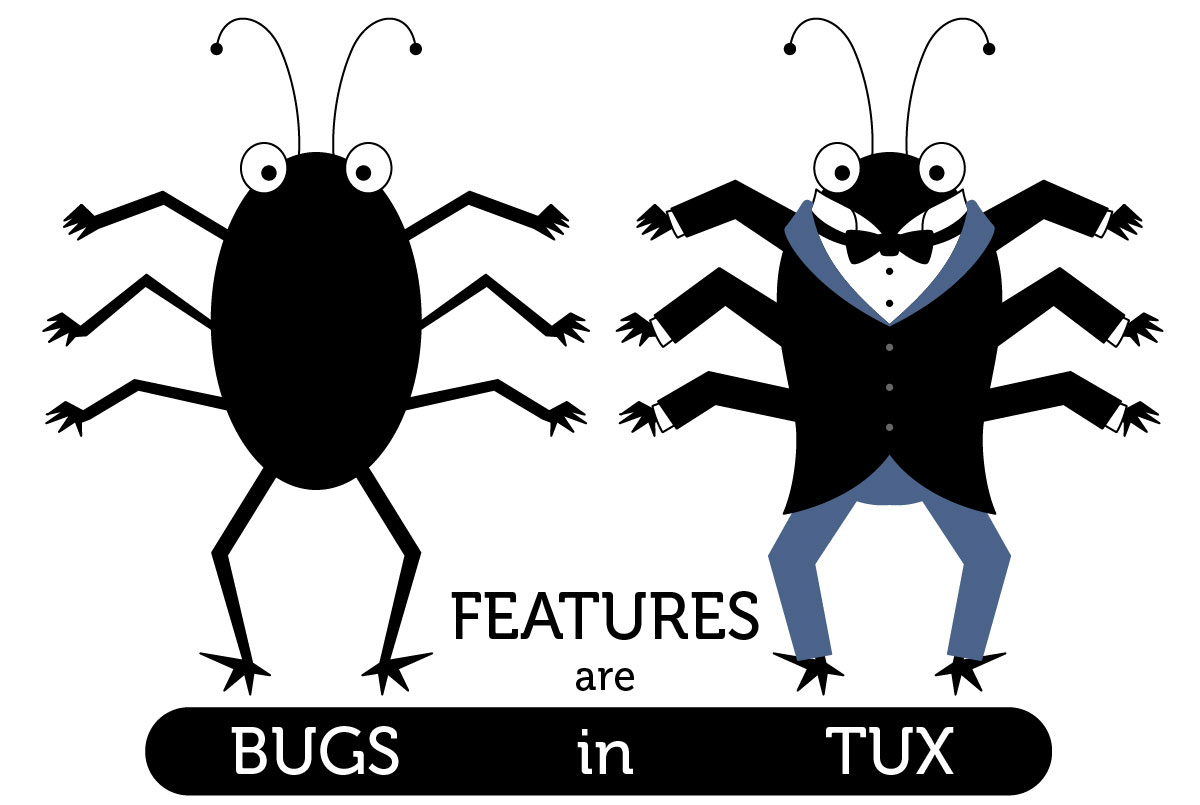
\includegraphics[width=.5\textwidth]{bugfeature.jpg}
\end{frame}
\begin{frame}[t]{The First Computer Bug}
    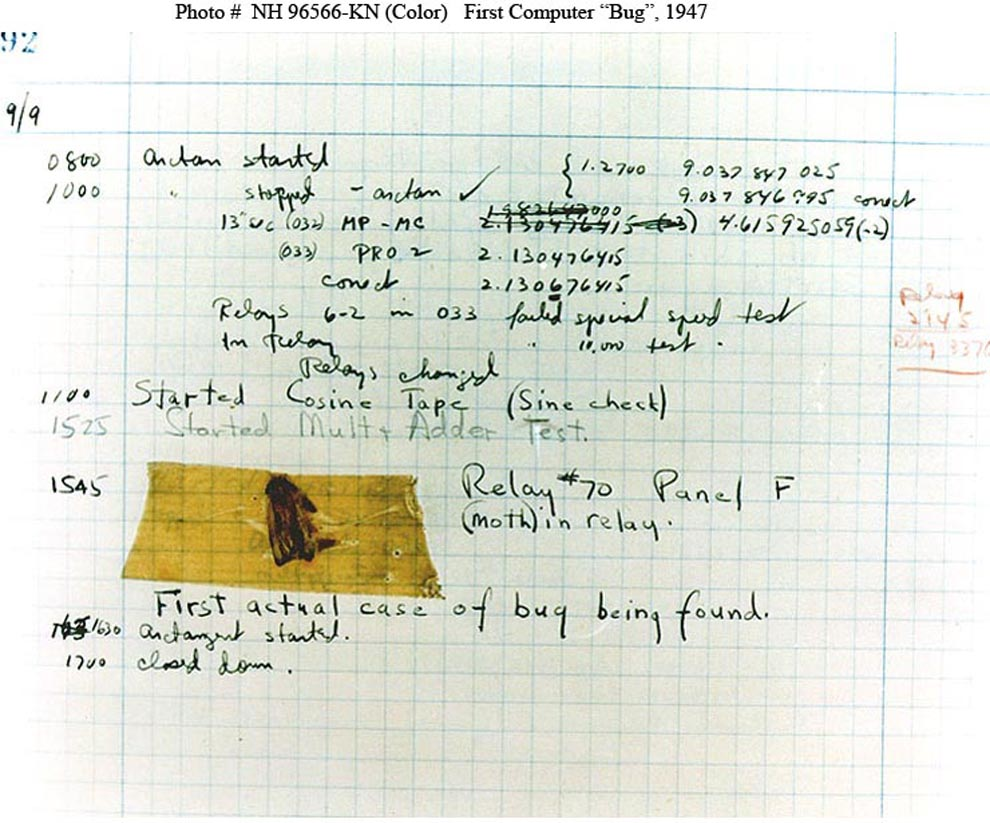
\includegraphics[width=.5\textwidth]{computer-bug.jpg}  
\end{frame}
\begin{frame}[t]{The First Computer Bug}
    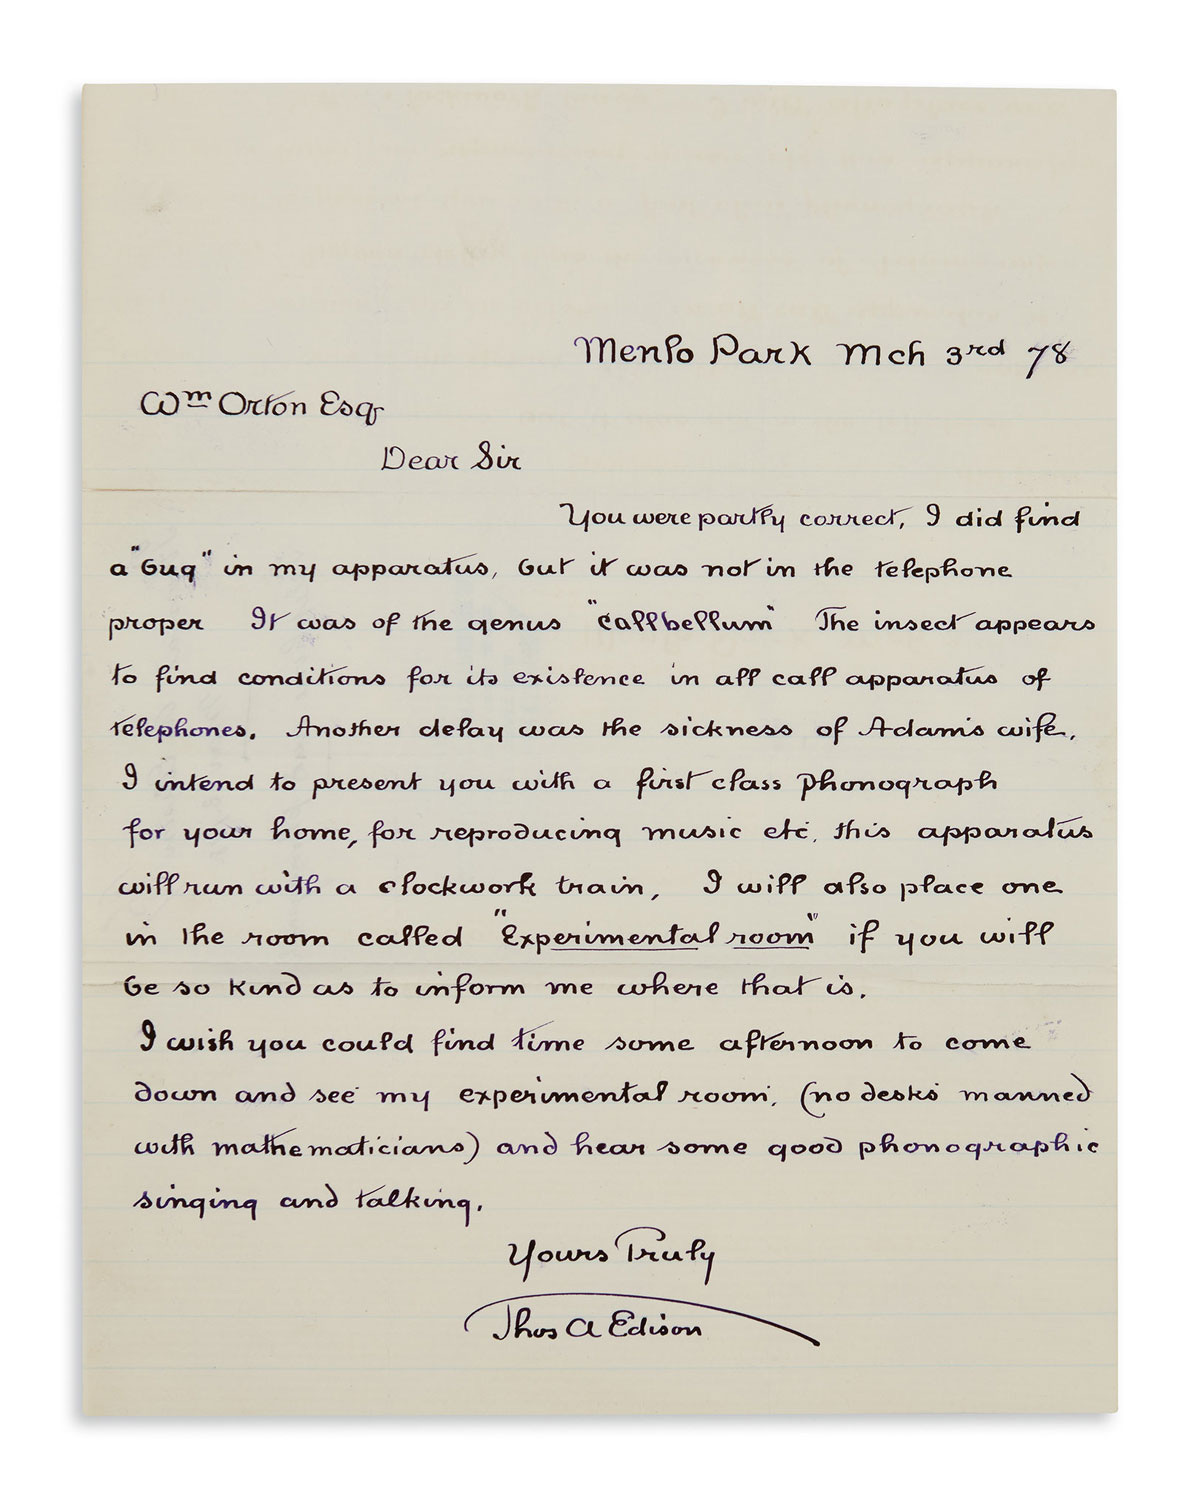
\includegraphics[width=.5\textwidth]{telebug.jpg}  
\end{frame}
\begin{frame}[t]{Combo}
    Combos were a design accident; lead producer Noritaka Funamizu noticed that extra strikes were possible during a bug check on the car-smashing bonus stage. He thought that the timing required was too difficult to make it a useful game feature, but left it in as a hidden one\footnote{\url{https://en.wikipedia.org/wiki/Combo_(video_games)}}.

    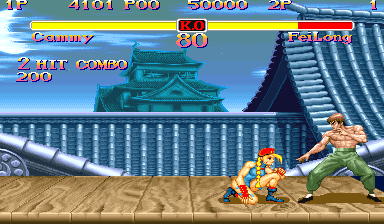
\includegraphics[width=.5\textwidth]{Super_Street_Fighter_II_screenshot.png}

\end{frame}

\begin{frame}[t]{彩蛋}
    
\includegraphics[width=.5\textwidth]{1280px-Konami_Code.svg.png} 
\end{frame}

\end{document}

